\documentclass{article}
\usepackage{setspace}
%\usepackage{subfigure}

\pagestyle{plain}
\usepackage{amssymb,graphicx,color}
\usepackage{amsfonts}
\usepackage{latexsym}
\usepackage{a4wide}
\usepackage{amsmath}
\usepackage{paper}
\usepackage{mathtools}
\usepackage{algorithm}
\usepackage{algpseudocode}
\usepackage{cfr-lm}
\newtheorem{theorem}{Theorem}
\newtheorem{lemma}[theorem]{Lemma}
\newtheorem{corollary}[theorem]{Corollary}
\newtheorem{proposition}[theorem]{Proposition}
\newtheorem{remark}[theorem]{Remark}
\newtheorem{definition}[theorem]{Definition}
\newtheorem{fact}[theorem]{Fact}

\newtheorem{problem}[theorem]{Problem}
\newtheorem{exercise}[theorem]{Exercise}
\def \set#1{\{#1\} }




\newenvironment{proof}{
PROOF:
\begin{quotation}}{
$\Box$ \end{quotation}}

\usepackage{xcolor}
\newcommand{\jk}[1]{{\color{blue} [JK: #1]}}
\newcommand{\jw}[1]{{\color{gray} [JW: #1]}}

\newcommand{\nats}{\mbox{\( \mathbb N \)}}
\newcommand{\rat}{\mbox{\(\mathbb Q\)}}
\newcommand{\rats}{\mbox{\(\mathbb Q\)}}
\newcommand{\reals}{\mbox{\(\mathbb R\)}}
\newcommand{\ints}{\mbox{\(\mathbb Z\)}}
\newcommand{\Cat}{\operatorname{\mathcal{C}}}
\newcommand{\Chol}{\operatorname{Chol}}
\newcommand{\KLD}{\operatorname{\mathbb{D}_{\text{KL}}}}
\newcommand{\D}{\operatorname{\mathbb{D}}}
\newcommand{\WD}{\operatorname{\mathbb{D}_{W_2}}}
\newcommand{\tr}{\operatorname{tr}}
\newcommand{\diag}{\operatorname{diag}}
\newcommand{\GP}{\operatorname{\mathcal{GP}}}
\newcommand{\wc}{\operatorname{{}\cdot{}}}

\DeclareMathOperator*{\argmax}{arg\,max}
\DeclareMathOperator*{\argmin}{arg\,min}

% make sure equation numbers start with the section they are from
\numberwithin{equation}{section}
%%%%%%%%%%%%%%%%%%%%%%%%%%


\begin{document}

\onehalfspacing
\begin{titlepage}
	\centering
\begin{figure}[h!]
\begin{flushright}
    
\includegraphics[width=.333\textwidth]{ucl_logo.png}
\end{flushright}
\end{figure}
    {}
	\vspace{4.5cm}

	{\Huge\bfseries Generalised Variational Inference \\ for Gaussian Processes\par}
	% \vfill

	\vspace{1cm}
	{\Large\itshape James Wu\par}
	\vspace{0.5cm}
	supervised by\par 
	\vspace{0.25cm}
    Veit D. \textsc{Wild} \& Jeremias \textsc{Knoblauch}
	\vfill
	{\large September 2023\par}
	\vspace{2cm}
	% \vfill

% Bottom of the page
\end{titlepage}
\pagenumbering{gobble}
\newpage
\setcounter{page}{1}
\pagenumbering{roman}

This report is submitted as part requirement for the Master's in Computational Statistics \& Machine Learning Degree at University College London (UCL). It is substantially the result of my own work except where explicitly indicated in the text.

\begin{flushright}
    \textit{James (Jian Shu) Wu}
    
    September 2023
\end{flushright}
\newpage


\section*{Acknowledgements}
Thanks mom!
\newpage

\begin{abstract}
Summarise your report concisely.
\end{abstract}
\newpage
\tableofcontents
\newpage
\pagenumbering{arabic}
\setcounter{page}{1}
\section{GPs: Expressive but \textit{not Scaleable}}
Gaussian processes (GPs) are powerful universal function approximators that can be used for both regression and classification tasks. 
\subsection{The GP}\label{section:the-gp}
We introduce the GP following \cite{rasmussen2003gaussian}. For an input space $\mathcal{X}$, a GP is a random function mapping $F(\cdot)$ where a sample function $f(\cdot) \sim F(\cdot)$ applies the mapping $f: \mathcal{X} \rightarrow \mathbb{R}$ and $F(\cdot)$ follows:
\begin{align}
    P_{\GP}\left(F\left(\cdot \right)\right) =  \mathcal{N}(m^p(\cdot), k^p(\cdot, \cdot))
    \label{gp-normal}
\end{align}
defined with respect to a mean function $m^p: \mathcal{X} \rightarrow \mathbb{R}$ and a positive definite kernel function $k^p: \mathcal{X} \times \mathcal{X} \rightarrow \mathbb{R}$. In other words, for any $N$ points $\mathbf{X}_N = \left\{ x_n\right\}_{n=1}^N$ where $x_n \in \mathcal{X}$, a GP constructs the Gaussian distribution:
\begin{align}
    \label{gp-vector}
    P_{\GP}\left(F\left(\mathbf{X}_N\right)\right) = P_{\GP}\left(Y_N \vert \mathbf{X}_N\right) = \mathcal{N}\left(\mathbf{m}^p_{\mathbf{X}_N}, \mathbf{K}^{p}_{\mathbf{X}_N, \mathbf{X}_N}\right)
\end{align}
where $\mathbf{m}^p_{\mathbf{X}_N} = \left[ m^p(x_1) \cdots m^p(x_N)\right]^T \in \mathbb{R}^N$, $\mathbf{K}^p_{\mathbf{X}_N, \mathbf{X}_N} \in \mathbb{R}^{N \times N}$ having elements:
\begin{align}
    \left[\mathbf{K}^p_{\mathbf{X}_N, \mathbf{X}_N}\right]_{n, n'} = k^p(x_n, x_{n'})
\end{align}
for $n, n'=1,\dots, N$, and $Y_N \in \mathbb{R}^{N}$ is the random response vector corresponding to $F(\mathbf{X}_N)$. Bold font $\mathbf{X}_N$ and $\mathbf{Y}_N$ will be a shorthand for denoting known vectors or matrices of the form $\mathbf{X}_N = \left\{ x_n\right\}_{n=1}^N$ and $\mathbf{Y}_N = \left\{ y_n\right\}_{n=1}^N$ respectively. $X_N$ and $Y_N$ will denote random vectors or matrices with respect to $N$ points.

In both regression and classification tasks, GPs are a powerful modelling approach. Minimal restrictions for choosing the mean function $m^p: \mathcal{X} \rightarrow \mathbb{R}$ and positive definite kernel function $k^p: \mathcal{X} \times \mathcal{X} \rightarrow \mathbb{R}$ in (\ref{gp-normal}) provide endless possibilities for constructing expressive GP model spaces. This control and visibility into the model's behaviour, is a strong advantage of GPs compared to other modelling approaches. 

\cite{novak2019neural} shows that the GP is an important construction for understanding the theoretical properties of many Bayesian neural network architectures. Showing that the infinite width limit of many such architectures can be expressed as a GP has provided a theoretical framework for analysing neural networks typically viewed as black box approaches. This provides further motivation for the potential and importance of GPs.

\subsection{GP Regression}
Consider the regression task where we have $N$ observation pairs $\left\{(x_n, y_n)\right\}_{n=1}^{N}$ with inputs $x_n \in \mathcal{X}$ and responses $y_n \in \mathbb{R}$. GP regression models the data generating process:
\begin{align}
    y_n \sim F(x_n) + E
    \label{regression-data-uncertainties}
\end{align}
where the GP random function mapping $F(\cdot)$ accounts for the epistemic (model) uncertainty and the random scalar $E$ accounts for the aleatoric (measurement) uncertainty. In this formulation, we assume that the aleatoric uncertainty is homoscedastic of the form:
\begin{align}
    E = \mathcal{N} \left(0, \sigma^2\right)
    \label{aleotric-uncertainty}
\end{align}
GP regression uses the formulation in Section \ref{section:the-gp} to `predict' for $N^*$ test points $\mathbf{X}_{N*} = \left\{ x_{n^*}\right\}_{n^*=1}^{N^*}$ with a Bayesian posterior. (\ref{gp-vector}) provides the prior for the response vector of the test points:
\begin{align}
    \label{gp-prior}
    P_{\GP}\left(Y_{N*}\vert \mathbf{X}_{N*}\right) = \mathcal{N}\left(\mathbf{m}^p_{\mathbf{X}_{N*}}, \mathbf{K}^p_{\mathbf{X}_{N*}, \mathbf{X}_{N*}}\right)
\end{align}
Evaluating the known training response vector $\mathbf{Y}_{N}$ provides the multi-variate Gaussian likelihood:
\begin{align}
     \label{gp-likelihood}
    P_{\GP}\left(\mathbf{Y}_{N} \vert \mathbf{X}_{N} \right) = \left(2 \pi\right)^{-N/2} \det\left(\mathbf{K}^p_{\mathbf{X}_{N}, \mathbf{X}_{N}}\right)^{-1/2} \exp\left(-\frac{1}{2}\left(\mathbf{e}^p_N\right)^T\left(\mathbf{K}^p_{\mathbf{X}_{N}, \mathbf{X}_{N}}\right)^{-1}\mathbf{e}^p_N\right)
    \label{likelihood-normal}
\end{align}
defining:
\begin{align}
    \mathbf{e}^p_N \coloneqq \left(\mathbf{Y}_N - \mathbf{m}^p_{\mathbf{X}_{N}} \right)
    \label{mean-error-definition}
\end{align}
With Bayes' Rule, the posterior of the response vector is proportional to the prior and likelihood:
\begin{align}
     P_{\GP}\left(Y_{N*} | \mathbf{Y}_{N},  \mathbf{X}_{N},  \mathbf{X}_{N*}\right) \propto P_{\GP}\left(\mathbf{Y}_{N} \vert \mathbf{X}_{N} \right) P_{\GP}\left(Y_{N*}\vert \mathbf{X}_{N*}\right)
    \label{bayes-posterior}
\end{align}
In GP regression, the posterior in (\ref{bayes-posterior}) acts as a `prediction' for the epistemic uncertainty of the test data responses. With all terms being Gaussian, the posterior in (\ref{bayes-posterior}) has the form:
\begin{align}
    P_{\GP}\left(Y_{N*} | \mathbf{Y}_{N},  \mathbf{X}_{N},  \mathbf{X}_{N*}\right)  =  \mathcal{N}\left(\hat{\mathbf{m}}^p_{\mathbf{X}_{N*}}, \hat{\mathbf{K}}^p_{\mathbf{X}_{N*}, \mathbf{X}_{N*}}\right)
    \label{gp-epistemic-posterior}
\end{align}
with:
\begin{align}
    \label{gp-epistemic-posterior-mean}
    \hat{\mathbf{m}}^p_{\mathbf{X}_{N*}} = \mathbf{m}^p_{\mathbf{X}_{N*}} + \mathbf{K}^p_{\mathbf{X}_{N*}, \mathbf{X}_N} \left(\mathbf{K}^p_{\mathbf{X}_N, \mathbf{X}_N}\right)^{-1} \left( \mathbf{Y}_N - \mathbf{m}^p_{\mathbf{X}_N}\right)
\end{align}
and
\begin{align}
    \label{gp-epistemic-posterior-covariance}
    \hat{\mathbf{K}}^p_{\mathbf{X}_{N*}, \mathbf{X}_{N*}} = \mathbf{K}^p_{\mathbf{X}_{N*}, \mathbf{X}_{N*}} - \mathbf{K}^p_{\mathbf{X}_{N*}, \mathbf{X}_N}\left(\mathbf{K}^p_{\mathbf{X}_N, \mathbf{X}_N}\right)^{-1}\mathbf{K}^p_{\mathbf{X}_N, \mathbf{X}_{N*}}
\end{align}
With the aleoteric data uncertainty also modelled as a Gaussian in (\ref{aleotric-uncertainty}), GP regression models the test data responses in the closed form:
\begin{align}
    \mathbf{Y}_{N*} \sim P_{\GP}\left(Y_{N*} \vert \mathbf{Y}_N, \mathbf{X}_N, \mathbf{X}_{N*}, \sigma^2\right)
    \label{gp-posterior}
\end{align}
This is the GP predictive posterior where:
\begin{align}
    P_{\GP}\left(Y_{N*} \vert \mathbf{Y}_N, \mathbf{X}_N, \mathbf{X}_{N*}, \sigma^2\right) = \mathcal{N}\left(\bar{\mathbf{m}}^p_{\mathbf{X}_{N*}}, \bar{\mathbf{K}}^p_{\mathbf{X}_{N*}, \mathbf{X}_{N*}}\right)
    \label{gp-posterior-normal}
\end{align}
with:
\begin{align}
    \label{gp-posterior-mean}
    \bar{\mathbf{m}}^p_{\mathbf{X}_{N*}} = \mathbf{m}^p_{\mathbf{X}_{N*}} + \mathbf{K}^p_{\mathbf{X}_{N*}, \mathbf{X}_N} \left( \mathbf{K}^{p, \sigma^2}_{\mathbf{X}_N, \mathbf{X}_N}\right)^{-1} \left( \mathbf{Y}_N - \mathbf{m}^p_{\mathbf{X}_N}\right)
\end{align}
and
\begin{align}
    \label{gp-posterior-covariance}
    \bar{\mathbf{K}}^p_{\mathbf{X}_{N*}, \mathbf{X}_{N*}} = \mathbf{K}^p_{\mathbf{X}_{N*}, \mathbf{X}_{N*}} - \mathbf{K}^p_{\mathbf{X}_{N*}, \mathbf{X}_N}\left( \mathbf{K}^{p, \sigma^2}_{\mathbf{X}_N, \mathbf{X}_N}\right)^{-1}\mathbf{K}^p_{\mathbf{X}_N, \mathbf{X}_{N*}}
\end{align}
defining:
\begin{align}
    \mathbf{K}^{p, \sigma^2}_{\mathbf{X}_N, \mathbf{X}_N} \coloneqq \mathbf{K}^p_{\mathbf{X}_N, \mathbf{X}_N} + \sigma^2 \mathbf{I}_N
    \label{gp-covariance-with-sigma}
\end{align}
where $\mathbf{I}_N \in \mathbb{R}^{N \times N}$ is the identity matrix.

\subsection{GP Classification}\label{section:gp-classifiers}
Consider the classification task where we have $N$ observation pairs $\left\{(x_n, y_n)\right\}_{n=1}^{N}$ with inputs $x_n \in \mathcal{X}$ and responses $y_n \in \{1, \dots, J\}$. In other words, we wish to map each input $x_n$ to one of $J$ labels. Following the GP classification approach from \cite{matthews2017scalable}, we first construct a GP regression model for each label such that for a test point $x_n \in \mathcal{X}$, the posterior prediction is Gaussian:
\begin{align}
    y_n^j \sim \mathcal{N}\left(\bar{m}^p_j(x_n), \bar{k}^p_j(x_n, x_n)\right)
    \label{gp-classifier-regressors}
\end{align}
where $j=1, \dots, J$, defining $J$ i.i.d. random responses.
Concatenating $\mathbf{y}_n^{1:J} = [y_n^1 \cdots y_n^J]^T \in \mathbb{R}^{J}$, this real-valued random response vector is mapped to one of $J$ labels through a series of operations to construct the GP classifier:
\begin{align}
\label{gp-classifier}
y_n \sim \Cat \left(s\left(\mathbf{y}_n^{1:J}\right)\right) \\
y_n \sim \Cat \left(\mathbf{c}^p\right)
\label{gp-classifier}
\end{align}
where $y_n \in \{1, \dots, J\}$, the desired label response behaviour. This approach requires choosing $s: \mathbb{R}^J \rightarrow \Delta(J)$, a mapping from a $J$ dimensional real vector to a $J$ dimensional probability simplex $\mathbf{c}^p \in \Delta(J)$ which is used to parameterise a categorical distribution $\Cat$ (a generalisation of the Bernoulli distribution to $J$ labels).

\subsubsection{The Robust Max Function}\label{section:robust-max=function}
\cite{matthews2017scalable} provides a few different choices for defining the mapping $s: \mathbb{R}^J \rightarrow \Delta(J)$ in (\ref{gp-classifier}). We follow \cite{wild2022generalized}, using the robust max function to define the $j^{th}$ element of the probability simplex $\mathbf{c}^p$:
\begin{align}
c^p_j = s_{robust, j}^{(\epsilon)}\left(\mathbf{y}_n^{1:J}\right) = \begin{cases}
      1-\epsilon, &  \text{if } j = \arg \max\left(\mathbf{y}_n^{1:J}\right) \\
      \frac{\epsilon}{J-1}, & \text{otherwise} \\
   \end{cases}
   \label{robust-max-function}
\end{align}
where $\epsilon \in [0, 1]$. Typically, $\epsilon$ is chosen as a very small value (i.e. $1e^{-2}$). Constructing the $\Delta(J)$ vector with (\ref{robust-max-function}), we have the probability value of $1-\epsilon$ for the label of maximum value and $\frac{\epsilon}{J-1}$ otherwise. This formulation provides robustness to outliers, as it only considers the ranking of the GP models for each label.

A benefit of the robust max function is that the expected log-likelihood under the categorical distribution in (\ref{gp-classifier}), becomes analytically tractable. \cite{wild2022generalized} shows that with $N$ input and response pairs $\{x_n, y_n\}_{n=1}^N$:
\begin{align}
    \mathbb{E}_{P} \left[\log P\left(y \vert x\right)\right] \approx \sum_{n=1}^N \log(1-\epsilon) S^p(x_n, y_n) + \log\left(\frac{\epsilon}{J-1}\right) \left(1-S^p(x_n, y_n)\right)
    \label{robust-max-function-expected-log-likelihood}
\end{align}
with $P$ being the distribution in (\ref{gp-classifier}) and 
\begin{align}
    S^p(x_n, j) \coloneqq \frac{1}{\sqrt{\pi}}\sum_{i=1}^{I} w_i \left(\prod_{j'=1, j'\neq j}^J \phi\left(\frac{\xi_i\sqrt{(2 \bar{k}_{j'}^p(x_n, x_n)}+\bar{m}_{j}^p(x_n) - \bar{m}_{j'}^p(x_n)}{\sqrt{\bar{k}_{j'}^p(x_n, x_n)}}\right)\right)
\end{align}
where $\left\{w_i, \xi_i\right\}_{i=1}^I$ are respectively the weights and roots of the Hermite polynomial of order $I \in \mathbb{N}$. $\phi(\cdot)$ is the standard normal cumulative distribution function. This analytical expression can be used for inference on GP classifier parameters when defining a loss objective with respect to the log-likelihood.

\subsection{GPs aren't Scaleable}\label{section:gp-problems}
A major drawback of GPs has been their inability to scale with respect to $N$, the number of training points. Both classification and regression relies on evaluating the inversion of an $\mathbb{R}^{N \times N}$ matrix in (\ref{gp-posterior-mean}) and (\ref{gp-posterior-covariance}). This operation has computational complexity $\mathcal{O}(N^3)$ and space complexity $\mathcal{O}(N^2)$, both of which quickly become problematic when scaling to larger-sized training sets. Despite their impressive performance and theoretically-driven approach, the computational intractability of GPs has been a serious limitation, restricting their use to problem domains having smaller sized data sets. In Section \ref{section:the-svgp}, we will present sparse variational Gaussian Processes (svGPs), a well-known approach to scaling GPs to larger data sets.

\newpage
\section{svGPs: Scaleable but \textit{not Expressive}}\label{section:the-svgp}
Proposed by \cite{titsias2009variational}, sparse variational Gaussian Processes (svGPs) are a well-known approach to ensuring computational tractability when scaling GPs. We will review this approach followed by a discussion of its strengths and weaknesses.

\subsection{The svGP}
The svGP has the form:
\begin{align}
g(\cdot) \sim Q^{(\gamma)}_{\GP}(G(\cdot)) = \mathcal{N}\left(m^{q}(\cdot), k^{q}(\cdot, \cdot)\right)
\label{svgp}
\end{align}
parameterised by $\gamma$ which includes a subset of inducing points $\mathbf{X}_M = \{x_m\}_{m=1}^{M} \subset \{x_n\}_{n=1}^{N}$. For $N^*$ test points $\mathbf{X}_{N*}$, the svGP approximates the predictive posterior:
\begin{align}
    \mathbf{Y}_{N*} \sim Q_{\GP}^{(\gamma)}\left(Y_{N*} \vert \mathbf{X}_{N*}\right)
\end{align}
where:
\begin{align}
    Q_{\GP}^{(\gamma)}\left(Y_{N*} \vert \mathbf{X}_{N*}\right) = \mathcal{N}\left(\bar{\mathbf{m}}_{\mathbf{X}_{N*}}^{q}, \bar{\mathbf{K}}_{\mathbf{X}_{N*}, \mathbf{X}_{N*}}^{q}\right)
\end{align}
\cite{titsias2009variational} proposes an approximate predictive posterior mean function parameterised by a vector $\boldsymbol{\mu} \in \mathbb{R}^M$:
\begin{align}
    \label{svgp-mean} 
    \bar{\mathbf{m}}_{\mathbf{X}_{N*}}^{q} = \mathbf{m}^p_{\mathbf{X}_{N*}} + \mathbf{K}^p_{\mathbf{X}_{N*}, \mathbf{X}_M}\left(\mathbf{K}^p_{\mathbf{X}_M,\mathbf{X}_M}\right)^{-1} \boldsymbol{\mu}
\end{align}
and a kernel function parameterised by a positive definite matrix $\mathbf{\Sigma} \in \mathbb{R}^{M\times M}_{\succ 0}$:
\begin{align}
\bar{\mathbf{K}}_{\mathbf{X}_{N*}, \mathbf{X}_{N*}}^{q} & = \mathbf{K}^p_{\mathbf{X}_{N*}, \mathbf{X}_{N*}} - \mathbf{K}^p_{\mathbf{X}_{N*}, \mathbf{X}_M} \left(\mathbf{K}^p_{\mathbf{X}_M, \mathbf{X}_M}\right)^{-1}\mathbf{K}^p_{\mathbf{X}_M, \mathbf{X}_{N*}} \nonumber \\
&\qquad + \mathbf{K}^p_{\mathbf{X}_{N*}, \mathbf{X}_M}  \left(\mathbf{K}^p_{\mathbf{X}_M, \mathbf{X}_M}\right)  ^{-1} \mathbf{\Sigma} \left(\mathbf{K}^p_{\mathbf{X}_M, \mathbf{X}_M}\right)^{-1}\mathbf{K}^p_{\mathbf{X}_M, \mathbf{X}_{N*}}
\label{svgp-covariance}
\end{align}
All together, these define the parameter space:
\begin{align}
    \mathbf{\Gamma} = \left\{\boldsymbol{\mu} \in \mathbb{R}^{M}, \mathbf{\Sigma} \in \mathbb{R}^{M\times M}_{\succ 0}, \mathbf{X}_M = \left\{x_m\right\}_{m=1}^{M} \subset \{x_n\}_{n=1}^{N}\right\}
    \label{svgp-parameter-space}
\end{align}
We wish to find $\gamma^* \in \mathbf{\Gamma}$ such that for any test points $\mathbf{X}_{N*}$ the svGP approximates the exact posterior distribution from ($\ref{bayes-posterior}$):
\begin{align}
    P_{\GP}\left(Y_{N*} \vert \mathbf{X}_{N*}, \mathbf{Y}_N, \mathbf{X}_N, \sigma^2 \right) \approx Q_{\GP}^{(\gamma^*)}\left(Y_{N*} \vert \mathbf{X}_{N*}\right)
    \label{svgp-desired-approximation}
\end{align}
To approximate the exact predictive posterior, \cite{titsias2009variational} targets matching $L_{\ell \ell}$, the log-likelihood of $P_{\GP}$, with respect to the approximation parameter $\gamma \in \boldsymbol{\Gamma}$:
\begin{align}
    L_{\ell \ell} &= \log P_{\GP}\left(\mathbf{Y}_N \vert \mathbf{X}_N, \sigma^2\right) \\ 
     \label{log-like}
    &= \log \int_{\mathbb{R}^{N^*}} P_{\GP}\left(\mathbf{Y}_N, Y_{N*} \vert \mathbf{X}_{N}, \mathbf{X}_{N*}, \sigma^2\right) d Y_{N*} \\
     \label{log-like-approx-gp}
&= \log \int_{\mathbb{R}^{N^*}} Q^{(\gamma)}_{\GP}\left(Y_{N*} \vert \mathbf{X}_{N*}\right) \frac{P_{\GP}\left(\mathbf{Y}_N, Y_{N*} \vert \mathbf{X}_{N}, \mathbf{X}_{N*}, \sigma^2\right)}{Q^{(\gamma)}_{\GP}\left(Y_{N*} \vert \mathbf{X}_{N*}\right)} d Y_{N*}\\
&\geq \int_{\mathbb{R}^{N^*}} Q^{(\gamma)}_{\GP}\left(Y_{N*} \vert \mathbf{X}_{N*}\right) \log\left(\frac{P_{\GP}\left(\mathbf{Y}_N, Y_{N*} \vert \mathbf{X}_{N}, \mathbf{X}_{N*}, \sigma^2\right)}{Q^{(\gamma)}_{\GP}\left(Y_{N*} \vert \mathbf{X}_{N*}\right)} \right)d Y_{N*}
 \label{elbo-jensen}
 \\ & \qquad \eqqcolon L_{free}(\gamma)
 \label{elbo-definition}
\end{align}
where we introducing the approximate posterior in (\ref{log-like-approx-gp}) and lower bound the log-likelihood with Jensen's inequality in (\ref{elbo-jensen}). $L_{free}(\gamma)$ is known as the free energy or evidence lower bound (ELBO). Given that we can decompose:
\begin{align}
    P_{\GP}\left(\mathbf{Y}_N, Y_{N*} \vert \mathbf{X}_{N}, \mathbf{X}_{N*}, \sigma^2\right) = P_{\GP} \left(\mathbf{Y}_N \vert \mathbf{X}_{N}, \sigma^2\right) P_{\GP}\left(Y_{N*}\vert \mathbf{X}_{N*}, \sigma^2 \right)
    \label{decomposed-numerator}
\end{align}
we can rewrite:
\begin{align}
    L_{free}(\gamma) &= \int_{\mathbb{R}^{N^*}} Q^{(\gamma)}_{\GP}(Y_{N*} \vert \mathbf{X}_{N*}) \log \left(P_{\GP}\left(\mathbf{Y}_N \vert \mathbf{X}_{N}, \sigma^2\right)\right) d Y_{N*} \nonumber
    \\ & \qquad + \int_{\mathbb{R}^{N^*}} Q^{(\gamma)}_{\GP}(Y_{N*} \vert \mathbf{X}_{N*}) \log \left(\frac{P_{\GP}\left( Y_{N*} \vert \mathbf{X}_{N*}, \sigma^2\right) }{Q^{(\gamma)}_{\GP}\left(Y_{N*} \vert \mathbf{X}_{N*}\right)}\right) d Y_{N*}
    \label{elbo-broken-down}
\end{align}
for the Variational Inference loss objective:
\begin{align}
    \label{bvi-loss}
    L_{free}(\gamma) &=\mathbb{E}_{Q^{(\gamma)}_{\GP}}\left[\frac{1}{N}\sum_{n=1}^N\log \left(P_{\GP}\left(y_n \vert x_n, \sigma^2\right)\right)\right] \nonumber \\
    & \qquad - \KLD \left[Q^{(\gamma)}_{\GP}\left(Y_{N*} \vert \mathbf{X}_{N*}\right), P_{\GP}\left( Y_{N*} \vert \mathbf{X}_{N*}, \sigma^2\right) \right]
\end{align}
where $\KLD[\wc, \wc]$ is the Kullback Leibler (KL) divergence. In this set-up the KL divergence has the closed-form:
  \begin{multline}
    \KLD \left[Q^{(\gamma)}_{\GP}\left(Y_{N*} \vert \mathbf{X}_{N*}\right), P_{\GP}\left( Y_{N*} \vert \mathbf{X}_{N*}, \sigma^2\right) \right] \\
    = \frac{1}{2}\left( \tr\left(\left(\mathbf{K}^{p, \sigma^2}_{\mathbf{X}_M, \mathbf{X}_M}\right)^{-1} \boldsymbol{\Sigma}\right) - M +
    \left(\mathbf{m}^p_{\mathbf{X}_m} - \boldsymbol{\mu}\right)^T \left(\mathbf{K}^{p, \sigma^2}_{\mathbf{X}_M, \mathbf{X}_M}\right)^{-1} \left(\mathbf{m}^p_{\mathbf{X}_m} - \boldsymbol{\mu}\right)+ \log\left(\frac{\det\left(\mathbf{K}^{p, \sigma^2}_{\mathbf{X}_M, \mathbf{X}_M}\right)}{\det\left(\boldsymbol{\Sigma}\right)}\right) \right)
    \label{kld-closed-form}
  \end{multline}
\cite{titsias2009variational} shows that for a given set of inducing points $\mathbf{X}_M$, the optimal choices $\boldsymbol{\mu}^*$ and $\mathbf{\Sigma}^*$ to maximise (\ref{bvi-loss}) have the closed forms:
\begin{align}
    \label{svgp-optimal-mean}
    \boldsymbol{\mu}^* = \sigma^{-2}\mathbf{K}^p_{\mathbf{X}_M, \mathbf{X}_M}  \left(\mathbf{\Sigma}_M\right)^{-1}\mathbf{K}^p_{\mathbf{X}_M, \mathbf{X}_N}  \left(\mathbf{Y}_N - \mathbf{m}^p_{\mathbf{X}_N}\right)
\end{align}
and
\begin{align}
    \label{svgp-optimal-covariance}
    \mathbf{\Sigma}^* = \mathbf{K}^p_{\mathbf{X}_M, \mathbf{X}_M}  \left(\mathbf{\Sigma}_M\right)^{-1}\mathbf{K}^p_{\mathbf{X}_M, \mathbf{X}_M} 
\end{align}
where 
\begin{align}
    \mathbf{\Sigma}_M \coloneqq \mathbf{K}^p_{\mathbf{X}_M, \mathbf{X}_M}  + \sigma^{-2}\mathbf{K}^p_{\mathbf{X}_M, \mathbf{X}_N} \mathbf{K}^p_{\mathbf{X}_N, \mathbf{X}_M} 
    \label{svgp-optimal-sigma-m}
\end{align}
parameterising the approximate GP with:
\begin{align}
    \gamma = \left(\boldsymbol{\mu}^*, \mathbf{\Sigma}^*,  \mathbf{X}_M\right)
    \label{titsias-svgp-parameters}
\end{align}
This formulation ensures the matrix inversion of $\mathbb{R}^{M \times M}$ matrices having $\mathcal{O}\left(M^3\right)$ computational complexity and the operation $\mathbf{K}^p_{\mathbf{X}_M, \mathbf{X}_N} \mathbf{K}^p_{\mathbf{X}_N, \mathbf{X}_M} $ in (\ref{svgp-optimal-sigma-m}) having computational complexity $\mathcal{O}\left(NM^2\right)$. Thus, the computational complexity of this approach is $\mathcal{O}\left(NM^2\right)$ with space complexity $\mathcal{O}\left(NM\right)$. This significantly improves the scalability of GP approaches from the traditional GP in Section \ref{section:the-gp}. $M$ is typically chosen as $\mathcal{O}(N^{1/2})$ such that the svGP has $\mathcal{O}(N^{2})$ and $\mathcal{O}(N^{3/2})$ time and space complexity respectively.

\subsection{Inducing Points Selection}
Finding the inducing points $\mathbf{X}_M = \left\{x_m\right\}_{m=1}^{M} \subset \{x_n\}_{n=1}^{N}$ that optimise the variational objective $L_{free}(\gamma)$ in ($\ref{elbo-definition}$) can be computationally expensive \jw{citation needed}. \cite{burt2020convergence} proposes an iterative selection procedure that greedily chooses the next inducing point based on the highest marginal variance in the prior when conditioned on the currently selected set of inducing points:
\begin{align}
    \label{greedy-varaince-selection}
    \text{index}_{m+1} = \argmax \left(\diag \left(\mathbf{K}^p_{\mathbf{X}_N, \mathbf{X}_N} - \mathbf{K}^p_{\mathbf{X}_N, \mathbf{X}_{m}} \left(\mathbf{K}^p_{\mathbf{X}_{m}, \mathbf{X}_{m}}\right)^{-1}\mathbf{K}^p_{\mathbf{X}_{m}, \mathbf{X}_N}\right)\right)
\end{align}
where $m < M$, $\mathbf{X}_{m} \in \mathcal{X}^m$ are the $m$ inducing points already chosen, and $\text{index}_{m+1}$ is the index of the next inducing point.

Each element in the diagonal has computational complexity $\mathcal{O}(M^2)$ from matrix multiplication so looping over all $N$ candidate points along the diagonal is $\mathcal{O}(NM^2)$. The matrix inversion is $\mathcal{O}(M^3)$ but remains a constant when computing each element of the diagonal. Thus the complexity of selecting each inducing point is $\mathcal{O}(NM^2)$, assuming $M << N$. Repeating to select $M$ inducing points, this algorithm has $\mathcal{O}(NM^3)$ computational complexity.
\\\jw{Add other results from \cite{burt2020convergence}. Maybe any guarantees from this method?}
\\\jw{Maybe show a picture of the inducing points selected for a toy curve}

\subsection{svGPs aren't Expressive}\label{section:svgp-problems}
The svGP from \cite{titsias2009variational} provides a solution to the scaling issues of the GP but comes with its own drawback. The mean and kernel functions must now conform to the formulations of (\ref{svgp-mean}) and (\ref{svgp-covariance}) respectively. This approach defines an approximate GP space with respect to $\mathbf{\Gamma}$, which is quite limited compared to the original GP formulation. In the following sections, we will review the reasons for these restrictive mean and kernel functions as explained by \cite{matthews2017scalable}. This will introduce the link between GPs and Gaussian measures (GMs) on function spaces and the mis-match of support problem of the KL divergence on function spaces. 

\subsubsection{The Kolomogorov Extension Theorem}
The KL divergence in the Variational Inference objective (\ref{bvi-loss}) is vaguely defined. Divergences are defined with respect to probability measures that exist on a measurable space. Because GPs aren't probability measures, for a well-defined KL divergence between two GPs we need to first define corresponding measures on a measurable space. In other words, we need distributions on function spaces in order to compare distributions with a divergence.
Thus, we begin by reviewing the Kolmogorov Extension Theorem as presented by ... which guarantees a GP to have at least one GM formulation on a function space. 
\begin{theorem}[Kolmogorov Extension Theorem]
\label{kolomogorov-extension-theorem}
Given a finite space measure such that:
\begin{align}
    consistency 
    \label{kolomogorov-consistency}
\end{align}
Then there exists a probability measure on the product sigma algebra ... 
\begin{align}
    measure
    \label{kolomogorov-measure}
\end{align}
\end{theorem}
In other words, an object that satisfies the consistency requirements of (\ref{kolomogorov-consistency}) guarantees the existence of a corresponding measure on a function space. From (\ref{gp-vector}), we see that a GP will always generate a set of points which conform to a Gaussian distribution (i.e. for any $\mathbf{X}_{N*}$ the random response vector $Y_{N*}$ always follows a Gaussian), satisfying the consistency condition of (\ref{kolomogorov-consistency}). As such, the Kolmogorov Extension Theorem guarantees the existence of at least one GM corresponding to this GP in some measureable function space. 

\subsubsection{The Kullback-Leibler Divergence in Function Spaces}
Maximising $L_{free}$ in (\ref{bvi-loss}) with respect to $\gamma \in \mathbf{\Gamma}$ is equivalent to solving:
\begin{align}
    \gamma^* = \argmin_{\gamma \in \mathbf{\Gamma}} \left\{\KLD \left[ Q_{\GP}^{(\gamma)}\left(Y_{N*} \vert \mathbf{X}_{N*}\right) ,  P_{\GP}\left(Y_{N*} \vert \mathbf{X}_{N*}, \mathbf{Y}_N, \mathbf{X}_N, \sigma^2 \right) \right]\right\}
    \label{elbo-kld}
\end{align}
minimising the KL divergence between the approximate posterior and the exact Bayesian posterior, which is proportional to the numerator of (\ref{elbo-jensen}). 

Guaranteed by the Kolomogorov Extension Theorem, the corresponding GMs of these GPs can be trivially constructed over the space of all functions $\mathcal{F} = \left\{f: \mathbb{R}^{N^*} \rightarrow \mathbb{R} \right\}$. We can now more precisely construct  (\ref{elbo-kld}):
\begin{align}
    \label{kld-function-spaces}
    \gamma^* &=\argmin_{\gamma \in \mathbf{\Gamma}}  \left\{ \mathbb{D}_{\mathcal{F}, \text{\text{KL}}}\left[ \mathbb{Q}^{(\gamma)}_\mathcal{F},  \mathbb{P}^B_\mathcal{F}\right] \right\} \\
    &= \argmin_{\gamma \in \mathbf{\Gamma}} \left\{\int_{\mathcal{F}} \log \left( \frac{d \mathbb{Q}^{(\gamma)}_\mathcal{F}}{d \mathbb{P}^B_\mathcal{F}} (f)\right)d \mathbb{Q}^{(\gamma)}_\mathcal{F}(f) \right\}
    \label{radon-nikodym}
\end{align}
where we can now denote that the KL divergence is with respect to measures on $\mathcal{F}$. $\mathbb{Q}^{(\gamma)}_\mathcal{F}$ is the GM on $\mathcal{F}$ corresponding to $Q_{\GP}^{(\gamma)}\left(Y_{N*} \vert \mathbf{X}_{N*}\right)$, the approximate GP predictive posterior and $\mathbb{P}^B_\mathcal{F}$ is the GM on $\mathcal{F}$ corresponding to $P_{\GP}\left(Y_{N*} \vert \mathbf{X}_{N*}, \mathbf{Y}_N, \mathbf{X}_N, \sigma^2 \right)$, the exact GP Bayesian predictive posterior. Following the loss objective form in (\ref{bvi-loss}) we can also more precisely formulate the Variational Inference objective:
\begin{align}
    \gamma^* = \argmin \left\{ \mathbb{E}_{Q^{(\gamma)}_{\GP}}\left[\frac{1}{N}\sum_{n=1}^N\log \left(P_{\GP}\left(y_n \vert x_n, \sigma^2\right)\right)\right] + \mathbb{D}_{\mathcal{F}, \text{KL}} \left[\mathbb{Q}^{(\gamma)}_{\mathcal{F}}, \mathbb{P}_{\mathcal{F}} \right] \right\}
    \label{bvi-gm-loss}
\end{align}
where $\mathbb{P}_\mathcal{F}$ corresponds to $P_{\GP}\left(Y_{N*} \vert \mathbf{X}_{N*}, \sigma^2 \right)$, the GM of the exact GP prior.

Without other assumptions on the GP, we're unable to show the existence of corresponding GMs on more well-behaved function spaces. This means that standard Variational Inference for GPs can be viewed as a minimisation of the KL divergence between GMs on $\mathcal{F}$. \cite{matthews2017scalable} explains that the strict svGP formulation of (\ref{svgp-optimal-mean}) and (\ref{svgp-optimal-covariance}) from \cite{titsias2009variational} are necessary to ensure the existence of the Radon-Nikodym derivative $d \mathbb{Q}_\mathcal{F}/d \mathbb{P}_\mathcal{F}$ shown explicitly in (\ref{radon-nikodym}) to ensure valid KL divergences in (\ref{kld-function-spaces}) and (\ref{bvi-gm-loss}) with the closed form expression in (\ref{kld-closed-form}). In other words, the svGP approximation space is restrictive due to the problem of support mis-match for the KL divergence between GMs on $\mathcal{F}$.

\subsubsection{Variational Inference is the Root Cause}
Most existing approaches attempt to approximate an ill-defined KL divergence on $\mathcal{F}$ caused by approximate GP constructions that are not the svGP \jw{Need citation}. However, \cite{wild2022generalized} identifies that Variational Inference is the root cause of the restrictive svGP approximation space, as learning in this framework necessitates a KL divergence in $\mathcal{F}$. The next section will introduce Generalised Variational Inference (GVI) from \cite{knoblauch2022optimization}, a learning framework that does not depend on the KL divergence. \cite{wild2022generalized} shows that with GVI we can avoid the support mis-match problem and learn in richer GP approximation spaces.

\newpage
\section{Generalising Variational Inference for GPs}
This section reviews Generalised Variational Inference (GVI) as introduced by \cite{knoblauch2022optimization} in the context of GPs. We show that a variational approximation learned from (\ref{elbo-kld}) involving the KL divergence and Bayesian posterior can be interpreted as a special case within a more general learning framework. This is followed by a review of \cite{wild2022generalized} demonstrating the feasibility of GVI as a GP learning framework.

\subsection{Generalising the Bayesian Posterior}
Statistical modelling is traditionally focused on characterising an underlying data generation process. In a Bayesian context, the regression model $y_n \sim F(x_n) + E$ introduced in (\ref{regression-data-uncertainties}) has the prior belief:
\begin{align}
    P_{\GP}\left(Y_{N*}\vert \mathbf{X}_{N*}, \sigma^2\right) = \mathcal{N}\left(\mathbf{m}^p_{\mathbf{X}_{N*}}, \mathbf{K}^{p, \sigma^2}_{\mathbf{X}_{N*}, \mathbf{X}_{N*}}\right)
    \label{gp-prior-normal}
\end{align}
and likelihood:
\begin{align}
    P_{\GP}\left(\mathbf{Y}_N|\mathbf{X}_N, \sigma^2\right) = \left(2 \pi\right)^{-N/2} \det\left(\mathbf{K}^{p, \sigma^2}_{\mathbf{X}_{N}, \mathbf{X}_{N}}\right)^{-1/2} \exp\left(-\frac{1}{2}\left(\mathbf{e}^p_N\right)^T\left(\mathbf{K}^{p, \sigma^2}_{\mathbf{X}_{N}, \mathbf{X}_{N}}\right)^{-1}\mathbf{e}^p_N\right)
    \label{gp-likelihood-normal}
\end{align}
These are used to update our belief model: 
\begin{align}
\label{bayesian-posterior}
P_{\GP}\left(Y_{N*} \vert \mathbf{Y}_N, \mathbf{X}_N, \mathbf{X}_{N*}, \sigma^2 \right) &= \frac{P_{\GP}\left(\mathbf{Y}_N|\mathbf{X}_N, \sigma^2\right)P_{\GP}\left(Y_{N*}\vert \mathbf{X}_{N*}, \sigma^2\right)}{\int_{\mathbb{R}^{N}} P_{\GP}\left(Y_{N*} Y_N  \vert, \mathbf{X}_N, \mathbf{X}_{N*}, \sigma^2 \right) d Y_{N}} \\
\label{bayesian-posterior-definition}
&\eqqcolon P_{\GP}^B \left(Y_{N*} \vert\mathbf{X}_{N*}, \sigma^2 \right)
\end{align}
where $P_{\GP}^B \left(Y_{N*} \vert\mathbf{X}_{N*}, \sigma^2 \right)$ is the Bayesian posterior, an update on the prior belief of the data generation process. The validity of the Bayesian posterior belief update relies on assumptions concerning the prior, the likelihood, and tractability. However in practice, variational GP learning is motivated by predictive performance and computational tractability rather than correct model specification, often violating the assumptions necessary for a valid Bayesian belief learning framework.

\subsubsection{The Bayesian Interpretation Breaks}
Bayesian approaches involve careful selection of the model prior $P_{\GP}(Y_{N*}\vert \mathbf{X}_{N*})$, often with domain expertise. The prior is assumed to be well-specified and well-informed. However, correctly specifying $m^p(\cdot)$ and $k^p(\cdot, \cdot)$ to construct the GP prior is difficult. In practice, the hyper-parameters of the mean and kernel are learned through some loss minimisation procedure of the predictive posterior likelihood on the training data (i.e. negative log-likelihood minimisation).
Thus, it would no longer seem reasonable to view $P_{\GP}(Y_{N*}\vert \mathbf{X}_{N*})$ as a prior belief before observing the training data when we are working backwards and learning the prior mean and kernel with the training data itself.

 Bayesian inference assumes that $y_n \sim F(x_n) + E$, the data input/response relationship modelled for GP regression, is the true data generating process and therefore the data likelihood can be evaluated with $P_{\GP}\left(\mathbf{Y}_N \vert \mathbf{X}_N, \sigma^2\right)$. Model mis-specification can often occur in traditional Bayesian inference, but techniques such as hypothesis testing, residual analysis, and domain expertise can help guide the construction of a reasonably well-specified setting. However in practice, this GP regression model is generally selected for its predictive performance and the conveniences of working with Gaussians. Thus, the likelihood model in (\ref{gp-likelihood-normal}) is almost definitely mis-specified. 
 
It is assumed that the Bayesian posterior is analytically and computationally tractable or that it can be adequately approximated. Being in an exclusively Gaussian setting, the exact Bayesian posterior is analytically tractable as shown in (\ref{gp-posterior}) but is computationally intractable scaling with $\mathcal{O}(N^3)$ compute and $\mathcal{O}(N^2)$ space complexity, as discussed in Section \ref{section:gp-problems}. This motivates the Variation Inference approximations like \cite{titsias2009variational} reviewed in Section \ref{section:the-svgp}. More generally, we can depict the approximation by \cite{titsias2009variational} as solving for $Q_{\GP}^{(\gamma^*)} \in \boldsymbol{Q}_{\mathbf{\Gamma}}$ where:
\begin{align}
    \boldsymbol{Q}_{\boldsymbol{\Gamma}} \coloneqq \left\{Q_{\GP}^{(\gamma)}: \gamma \in \mathbf{\Gamma}\right\}
    \label{svgp-space}
\end{align}
the svGP approximation space defined with respect to the parameter space $\mathbf{\Gamma}$. Traditional variational inference involves solving for $Q_{\GP}^{(\gamma^*)} \in \boldsymbol{Q}_{\boldsymbol{\Gamma}}$ that approximates the Bayesian posterior in (\ref{bayesian-posterior}), by minimising some divergence between the two: 
\begin{align}
Q^{(\gamma^*)}_{\GP} = \argmin_{Q^{(\gamma)}_{\GP} \in \boldsymbol{Q}_{\boldsymbol{\Gamma}}}\D\left[Q_{\GP}^{(\gamma)}, P_{\GP}^B\right]
\end{align}
where in the case of standard variational inference as shown in (\ref{elbo-kld}), $\D$ is the KL divergence.
However, as discussed in Section \ref{section:svgp-problems}, $\boldsymbol{Q}_{\boldsymbol{\Gamma}}$ must be a restricted approximation space to ensure a valid KL divergence, sacrificing the expressiveness of the space and adequate approximations of $P_{\GP}^B$. Given that $\boldsymbol{Q}_{\boldsymbol{\Gamma}}$ is mostly chosen for computational convenience, it's no longer reasonable to assume that $Q_{\GP}^{(\gamma^*)}$ will be a good approximation of the Bayesian posterior.

With the Bayesian interpretation of Variational Inference often violating core Bayesian assumptions, \cite{knoblauch2022optimization} proposes the GVI framework, which moves away from the traditional focus on correct model specification. GVI contextualises the Bayesian posterior in a learning framework focused on optimisation for predictive performance, more in line with the priorities of GP inference in practice.

\subsubsection{The Generalised Variational Inference (GVI) Interpretation}
Interpreting the Bayesian posterior as a solution of an optimisation problem can provide a more reasonable interpretation of approximate GP posteriors like the svGP from \cite{titsias2009variational}. In particular, \cite{knoblauch2022optimization} shows that the Bayesian posterior $P_{\GP}^B$ solves a special case of the General Variational Inference (GVI) objective:
\begin{align}
Q_{\GP}^* = \argmin_{Q_{\GP} \in \boldsymbol{Q}_{\GP}} \left\{ \mathbb{E}_{Q_{\GP}}\left[\frac{1}{N}\sum_{n=1}^N \ell(y_n, x_n)\right] + \D\left[Q_{\GP}, P_{\GP}\right]\right\}
\label{general-posterior}
\end{align}
by choosing the negative log-likelihood loss:
\begin{align}
    \ell(y_n, x_n) = -\log P_{\GP}\left(y_n \vert x_n, \sigma^2\right)
\end{align}
the KL divergence between the corresponding GMs on $\mathcal{F}$:
\begin{align}
    \D \left[Q_{\GP}, P_{\GP}\right] = \mathbb{D}_{\mathcal{F}, \text{KL}}\left[\mathbb{Q}_{\mathcal{F}}, \mathbb{P}_{\mathcal{F}}\right]
\end{align}
and an unrestricted feasible set for $\boldsymbol{Q}_{\GP}$. Moreover, the solution is $Q_{\GP}^{(\gamma^*)}$ when restricting the feasible set to the svGP approximation space $\boldsymbol{Q}_{\boldsymbol{\Gamma}}$ recovering (\ref{bvi-loss}) and the optimal solution from \cite{titsias2009variational}. But no longer deriving the Bayesian posterior through a belief update, we are no longer required to approximate the exact Bayesian posterior as the inference target. Instead, $Q_{\GP}^*$ approximates a generalised posterior defined with respect to a choice of loss $\ell(y_n, x_n)$ and regulariser $\D\left[\wc, P_{\GP}\right]$. \cite{knoblauch2022optimization} re-interprets the role of the prior, likelihood, and approximation space, in the context of this optimisation framework.

The empirical risk: 
\begin{align}
\mathcal{E}(Q_{\GP}) = \mathbb{E}_{Q_{\GP}}\left[\frac{1}{N}\sum_{n=1}^N \ell\left(y_n, x_n\right)\right]
\label{empirical-risk}
\end{align}
is equivalent to the expectation term in the GVI objective of (\ref{general-posterior}). This shows that the negative log-likelihood is just a specific loss definition for empirical risk minimisation. Focusing on predictive performance rather than model specification, the validity of the generalised posterior solution no longer depends on a well-specified likelihood.

The prior $P_{\GP}$ only exists in the divergence term of (\ref{general-posterior}), defining a regulariser for empirical risk minimisation. Unlike in the Bayesian interpretation, $P_{\GP}$ is no longer required to be a well-specified prior. In this context, the choice of the prior and the discrepancy $\D$ controls model complexity and prevents overfitting to the empirical risk. This is a more appropriate interpretation of GP modelling in practice, where prior mis-specification is almost certainly guaranteed.

With the GVI interpretation, the Bayesian posterior becomes the minimiser of regularised empirical risk. This redefines $P_{\GP}^B$ as an optimal solution with respect to predictive performance rather than as the result of an often ill-posed belief update. By pivoting from the standard Bayesian interpretation of $P_{\GP}^B$, we no longer need to have a well-specified likelihood, prior, or approximation space in the Bayesian sense. This learning framework allows us to approximate general posteriors that no longer rely on the KL divergence. To choose new divergences, we review \cite{wild2022generalized}, which constructs GMs corresponding to GPs on more structured function spaces to define stable divergences that can replace the KL divergence.

\subsection{Gaussian Measures on Hilbert Spaces}
GMs are typically defined as a Lebesgue measure on a physical probability space $(\Omega, \mathcal{A}, \mathbb{P})$. \cite{matthews2017scalable} explains that there does not exist an infinite-dimensional equivalent to the Lebesgue measure, especially in a space like $\mathcal{F}$. This means that in most cases, we cannot assume that a  probability measure that exists in a finite-dimensional space will have an infinite-dimensional analog.

\cite{wild2022generalized} explains that we can define measures on a Hilbert space as push-forward measures $\mathbb{P}^{F}(A) \coloneqq \mathbb{P}(F^{-1}(H))$, through the mapping $F: \Omega \rightarrow \mathcal{H}$, where $F \in \mathcal{H}$ for all Borel-measurable $H \subset \mathcal{H}$. Moreover if $F$ is a Gaussian random element satisfying:
\begin{align}
    \langle F, h \rangle_\mathcal{H} \sim \mathcal{N}\left(\mu(F, h), \sigma^2(F, h)\right)
\label{gre}
\end{align}
then we can define the corresponding push-forward measure as a GM on the Hilbert space, $\mathbb{P}_{\mathcal{H}}$. In other words, $\mathbb{P}_{\mathcal{H}}$ exists if for any $h \in \mathcal{H}$, the inner product $\langle F, h \rangle_\mathcal{H}$ follows a Gaussian distribution defined with respect to $\mu(F, h)$ and $\sigma^2(F, h)$.

\cite{wild2022generalized} shows that $P_{\GP}$ can be specified as $\mathbb{P}_{\mathcal{L}^2}$ a GM on a Hilbert space of square-integrable functions $\mathcal{L}^2(\mathcal{X}, \rho, \mathbb{R})$ if the mean function satisfies:
\begin{align}
    \label{smooth-mean-function-condition}
    m^p(\cdot) \in \mathcal{L}^2(\mathcal{X}, \rho, \mathbb{R})
\end{align}
and the kernel function is a trace class kernel satisfying:
\begin{align}
    \int_{\mathcal{X}} k^p(x, x) d\rho(x) < \infty
    \label{trace-kernel-condition}
\end{align}
These conditions guarantee sample functions from the GP $f(\cdot) \sim F(\cdot)$ to have square-integrable paths, allowing for a corresponding GM $\mathbb{P}_{\mathcal{L}^2} \coloneqq \mathcal{N}(m^p, C^p)$ defined on $\mathcal{L}^2(\mathcal{X}, \rho, \mathbb{R})$ with the same mean $m^p$ and a covariance operator:
\begin{align}
    C^p(f(\cdot)) \coloneqq \int_{\mathcal{X}} k^p(\cdot, x')f(x')d \rho(x')
    \label{gm-covariance-operator}
\end{align}
for any function $f \in \mathcal{L}^2(\mathcal{X}, \rho, \mathbb{R})$. This ensures the existence of a corresponding GM on a structured Hilbert space, allowing for divergences between GMs that wouldn't have been possible in $\mathcal{F}$. 

\subsection{Gaussian Wasserstein Inference for GPs}
Having shown that a GP can exist as a GM on a Hilbert space, \cite{wild2022generalized} uses the GVI framework from \cite{knoblauch2022optimization} to modify the objective in (\ref{bvi-gm-loss}):
\begin{align}
    \label{gwi-objective}
    \gamma^* = \argmin_{\gamma \in \boldsymbol{\Gamma}}\left\{ \mathbb{E}_{Q^{(\gamma)}_{\GP}}\left[- \frac{1}{N}\sum_{n=1}^N \log P_{\GP}\left(y_n \vert x_n, \sigma^2\right) \right] + \D_{\mathcal{H}} \left[\mathbb{Q}^{(\gamma)}_{\mathcal{H}}, \mathbb{P}_{\mathcal{H}} \right]\right\}
\end{align}
where $\mathbb{Q}^{(\gamma)}_{\mathcal{H}}$ and $\mathbb{P}_{\mathcal{H}}$ are GMs on Hilbert spaces corresponding to $Q^{(\gamma)}_{\GP}$ and $P_{\GP}$ respectively. By shifting from a divergence on $\mathcal{F}$ to a divergence on $\mathcal{H}$ and using GVI which allows for any valid divergence $\mathbb{D}$, we are no longer restricted to the svGP from \cite{titsias2009variational}, which was necessary to ensure a valid $\KLD\left[\mathbb{Q}_{\mathcal{F}},  \mathbb{P}_{\mathcal{F}}\right]$. 

\cite{wild2022generalized} proposes replacing the KL divergence on $\mathcal{F}$ with the Wasserstein distance between GMs on a Hilbert space. For two GMs $\mathbb{P}_{\mathcal{L}^2} = \mathcal{N}(m^p, C^p)$ and $\mathbb{Q}^{(\gamma)}_{\mathcal{L}^2} = \mathcal{N}(m^q, C^q)$ on the Hilbert space $\mathcal{L}^2(\mathcal{X}, \rho, \mathbb{R})$, the squared 2-Wasserstein distance between $\mathbb{P}_{\mathcal{L}^2}$ and $\mathbb{Q}_{\mathcal{L}^2}$ on (seperable) Hilbert spaces is:
\begin{align}
    \label{wasserstein-distance}
    \mathbb{D}_{\mathcal{L}^2, \text{W}_2} \left[\mathbb{P}_{\mathcal{L}^2}, \mathbb{Q}^{(\gamma)}_{\mathcal{L}^2}\right]^2 = \| m^p - m^q\|_2^2 + \tr(C^p) + \tr(C^q) - 2 \cdot \tr \left[ \left( \left(C^p\right)^{\frac{1}{2}} \left(C^q\right) \left(C^p\right)^{\frac{1}{2}}\right)^{\frac{1}{2}}\right]
\end{align}
where $\tr$ is the trace of an operator and $\left(C^p\right)^{1/2}$ is the square root of the positive, self-adjoint operator $C^p$. 

This motivates the Gaussian Wasserstein Inference objective from \cite{wild2022generalized}:
\begin{align}
    \label{gwi-objective}
    L_{gwi}(\gamma) = \mathbb{E}_{Q_{\GP}}\left[- \frac{1}{N}\sum_{n=1}^N \log P_{\GP}\left(y_n \vert x_n, \sigma^2\right) \right] + \mathbb{D}_{\mathcal{L}^2, \text{W}_2} \left[\mathbb{P}_{\mathcal{L}^2}, \mathbb{Q}^{(\gamma)}_{\mathcal{L}^2}\right]^2
\end{align}
where the regularisation is now between GMs on $\mathcal{L}^2(\mathcal{X}, \rho, \mathbb{R})$. Most mean and kernel functions satisfy (\ref{smooth-mean-function-condition}) and (\ref{trace-kernel-condition}) ensuring the existence of $\mathbb{P}_{\mathcal{L}^2}$ and $\mathbb{Q}^{(\gamma)}_{\mathcal{L}^2}$, providing significantly more freedom in defining $Q^{(\gamma)}_{\GP}$ than the svGP approach from \cite{titsias2009variational}. With (\ref{gwi-objective}), \cite{wild2022generalized} trains GWI-net, constructing $Q^{(\gamma)}_{\GP}$ with a neural network mean function to replace the svGP mean in (\ref{svgp-mean}), showing the potential of this new approach.


\newpage
\section{GVI-GPs: Expressive \textit{and} Scaleable}
In this section, we present GVI-GPs (Generalised Variational Inference Gaussian Processes), GPs learned through the GVI framework.

\subsection{A General Framework for GP Learning}
Motivated by \cite{wild2022generalized} and the GVI framework from \cite{knoblauch2022optimization}, we propose the general objective for learning GVI-GPs:
\begin{align}
Q_{\GP}^* = \argmin_{Q_{\GP} \in \boldsymbol{Q}_{\mathcal{G}}} \left\{ \mathbb{E}_{Q_{\GP}}\left[\frac{1}{N}\sum_{n=1}^N \ell(y_n, x_n)\right] + \D_{\mathcal{G}}\left[\mathbb{Q}_{\mathcal{G}}, \mathbb{P}_{\mathcal{G}}\right]\right\}
\label{gvi-gp-objective}
\end{align}
where the prior GP must have a corresponding GM on the function space $\mathcal{G}$ and we define a general approximation space:
\begin{align}
    \boldsymbol{Q}_{\mathcal{G}} \coloneqq \left\{ 
    Q_{\GP} :  \exists \mathbb{Q}_{\mathcal{G}},  \D_{\mathcal{G}}\left[\mathbb{Q}_{\mathcal{G}}, \mathbb{P}_{\mathcal{G}}\right] < \infty
    \right\}
\end{align}
where $\mathbb{Q}_{\mathcal{G}}$ is a corresponding GM on $\mathcal{G}$ and $\D_{\mathcal{G}}\left[\mathbb{Q}_{\mathcal{G}}, \mathbb{P}_{\mathcal{G}}\right] < \infty$ indicates a valid divergence with respect to the regulariser $\D_{\mathcal{G}}[\wc, \mathbb{P}_{\mathcal{G}}]$. 

We can recover a general form of Gaussian Wasserstein Inference from \cite{wild2022generalized}, by choosing the squared 2-Wasserstein distance on $\mathcal{L}^2(\mathcal{X}, \rho, \mathbb{R})$ and the approximation space:
\begin{align}
    \boldsymbol{Q}_{\mathcal{L}^2} \coloneqq \left\{ 
    \left(m^q, k^q\right): m^q \in \mathcal{L}^2(\mathcal{X}, \rho, \mathbb{R}), \int_{\mathcal{X}} k^q(x, x)d\rho(x) < \infty
    \right\}
\end{align}
containing all valid mean and kernel functions that ensure the existence of a GM on $\mathcal{L}^2(\mathcal{X}, \rho, \mathbb{R})$. 

If we choose the mean parameter space $\mathbb{R}^M$ with the svGP mean function in (\ref{svgp-mean}) and the kernel parameter space $\mathbb{R}^{M\times M}_{\succ 0}$ with the kernel function in (\ref{svgp-covariance}) as well as the inducing points $\left\{x_m, y_m\right\}_{m=1}^{M} \subset \{x_n, y_n\}_{n=1}^{N}$, and approximation space $\boldsymbol{Q}_{\boldsymbol{\Gamma}}$, we can also recover the svGP from \cite{titsias2009variational}.

It is important to note that unlike $\boldsymbol{Q}_{\boldsymbol{\Gamma}}$, the space $\boldsymbol{Q}_{\mathcal{L}^2}$ is defined independently of the prior GP. This decoupling of the approximation space from the prior is only possible because of the connection between GPs and GMs on Hilbert spaces shown in \cite{wild2022generalized} and GVI from \cite{knoblauch2022optimization}. Thus depending on the divergence and function space, the approximation space $\boldsymbol{Q}_{\mathcal{G}}$ may not necessarily depend on the prior GP, which will be useful for defining more expressive approximation spaces.

In practice, we choose a subset:
\begin{align}
    \boldsymbol{Q}_{\boldsymbol{\Theta}} \coloneqq \left\{ 
    Q^{(\theta)}_{\GP}: \theta \in \boldsymbol{\Theta} 
    \right\} \subset \boldsymbol{Q}_{\mathcal{G}}
\end{align}
such that we can construct an optimisation strategy with respect to some finite hyper-parameter space $\boldsymbol{\Theta}$ for the mean and kernel functions:
\begin{align}
    \boldsymbol{\Theta} \coloneqq \left\{\theta^m \in \boldsymbol{\Theta}^m, \theta^k \in \boldsymbol{\Theta}^k \right\}
\end{align}
where $\boldsymbol{\Theta}^m$ is the mean function hyper-parameter space and $\boldsymbol{\Theta}^k$ is the kernel function hyper-parameter space. $\boldsymbol{Q}_{\boldsymbol{\Theta}}$ remains a very general and expressive GP approximation space. 
In Section \ref{section:gvi-gp-construction}, we present some choices for mean and variational kernel functions with corresponding hyper-parameter spaces $\boldsymbol{\Theta}^m$ and $\boldsymbol{\Theta}^k$ to construct $\boldsymbol{Q}_{\boldsymbol{\Theta}}$. 

$\boldsymbol{Q}_{\mathcal{G}}$ provides an expressive approximation space for GVI-GPs, with the potential to learn in complex problem domains traditionally dominated by neural network architectures.
By choosing variational kernels, we also ensure the scaleability of GVI-GPs. 
Section \ref{section:gvi-gp-construction} will also propose different choices of discrepancies and priors for the regulariser $\D_{\mathcal{G}}\left[\wc, \mathbb{P}_{\mathcal{G}}\right]$ and the loss $\ell(y_n, x_n)$ in (\ref{gvi-gp-objective}). This demonstrates the flexibility of GVI-GP learning to approximate general posteriors beyond the exact Bayesian posterior.

\subsection{The GVI-GP Training Procedure}

\begin{algorithm}
\caption{GVI-GP Training Procedure}\label{alg:gvi-gp}
\begin{algorithmic}
\begin{enumerate}
    \item Choose a prior GP construction.
    \item Train the prior GP and select the inducing points.
    \item Choose a GVI-GP construction.
    \item Construct a GVI-GP objective.
    \item Train the GVI-GP.
    \item Temper the GVI-GP.
\end{enumerate}
\end{algorithmic}
\end{algorithm}

\subsubsection{Prior GP Training and Inducing Points Selection}
\jw{describe chicken and egg problem}

\begin{algorithm}
\caption{Prior GP Training and Inducing Points Selection}\label{alg:gvi-gp}
\begin{algorithmic}
 \State Select the inducing points $\left\{x_m\right\}_{m=1}^{M} \subset \{x_n\}_{n=1}^{N}$ with the initial prior GP kernel.
\While{the inducing points have not converged}
\State Train the prior GP on selected inducing points and their responses $\left\{x_m, y_m\right\}_{m=1}^{M}$.
\State  Select new inducing points with the trained prior GP kernel.
\EndWhile
\end{algorithmic}
\end{algorithm}
\jw{incorporates response data into the inducing point selection through the empirical risk minimisation training process. previously, inducing point selection only looked at $\mathbf{X}_N$}

\subsubsection{Regression Tempering}
\subsubsection{Classification Tempering}

\newpage
\section{GVI-GP Construction}\label{section:gvi-gp-construction}
\subsection{Means}
\jw{
Neural Networks!!!

Leverage existing architectures that have proved successful in their respective problem domains. CNN for images, Fully connected for regression, transformers for text?

But technically can be anything, i.e. random forest, KNN, etc.
}

\subsection{Kernels}\label{section:kernels}
A common practical drawback of GP modelling are the traditionally available kernel functions when constructing GPs. More traditional kernels (i.e. squared exponential kernels, periodic kernels, etc) have few learnable hyper-parameters compared to highly parameterised neural networks. This can limit the performance of GPs in problem domains involving structured high-dimensional data like image or text data, even if the problem of scalability is ignored. In this section we review the NNGP kernels from \cite{novak2019neural} and also present a form of deep neural network kernels, both with potential applications in problem domains typically under-represented by GP approaches.

\subsubsection{Neural Network Gaussian Process (NNGP) Kernels}
\subsubsection{Neural Network Kernels}
Recommend using non-stationary base kernel to pass gradients through the kernel to the NN. 

For this model we use $P \sim \mathcal{N}(m^p, k) $ and $Q \sim \mathcal{N}(m_Q, r)$ with 
\begin{itemize}
    \item $m^p = 0$ and $k$ an infinite width nn-gp kernel
    \item The variational mean is a nn with $L \in \bbN$ hiden layers, i.e. 
    \begin{align}
        m_Q(x) = w^T \phi\big( h^{L}(x) \big)
    \end{align}
    where $\phi$ is a non-linearity and $h^L(x)$ die output of the $L$-th hidden layer. 
    \item 
    The variational kernel $r$ is defined as 
    \begin{align}
        r(x,x') := r_0(x,x') - r_0(x,Z) \big( r_0(Z,Z) \big)^{-1} r_0(Z,x)
    \end{align}
    with $r_0(x,x') = h^{L}(x)^T h^{L}(x')$.
\end{itemize}
Maybe you need to use some tricks for training. I.e. training a neural network mean first and then only later use the full loss $L$

\subsection{Variational Kernels}
\jw{All require the selection of inducing points $\mathbf{X}_M$. We want it to somehow mimic the posterior covariance behaviour of greater uncertainty around previously unseen data.}


\subsubsection{Extended svGP Kernels}
Inspired by the svGP kernel from \cite{titsias2009variational}:

\begin{align}
            \bar{\mathbf{K}}^q_{\mathbf{X}_{N*}, \mathbf{X}_{N*}} := \mathbf{K}^p_{\mathbf{X}_{N*}, \mathbf{X}_{N*}} - \mathbf{K}^p_{\mathbf{X}_{N*}, \mathbf{X}_M}\left(\mathbf{K}^p_{\mathbf{X}_{M}, \mathbf{X}_M}\right)^{-1}\mathbf{K}^p_{\mathbf{X}_M, \mathbf{X}_{N*}} + \mathbf{\Sigma}^{\zeroslash}_{\mathbf{X}_{N*}, \mathbf{X}_{N*}} 
\end{align}
where $\mathbf{\Sigma}^{\zeroslash}_{\mathbf{X}_{N*}, \mathbf{X}_{N*}} \in \mathbb{R}^{N^*\times N^*}_{\succ 0}$ is any positive definite matrix constructed with respect to the test points $\mathbf{X}_{N*}$ and parameterised by $\theta^k \in \boldsymbol{\Theta}^k$. \jw{Go over different paramterisations, i.e. diagonal, kernel, etc.}which can be chosen as any kernel from Section \ref{section:kernels} i.e. with a deep NN kernel or a NNGP kernel.

with $\mathcal{O}(M^3)$ computational complexity better than $\mathcal{O}(NM^2)$ of svGP kernel.


\subsubsection{Sparse Posterior Kernels}
Inspired by the GP posterior covariance in (\ref{gp-posterior-covariance}):
\begin{align}
            \bar{\mathbf{K}}^q_{\mathbf{X}_{N*}, \mathbf{X}_{N*}} := \mathbf{K}^{\zeroslash}_{\mathbf{X}_{N*}, \mathbf{X}_{N*}} - \mathbf{K}^{\zeroslash}_{\mathbf{X}_{N*}, \mathbf{X}_M} \left( \mathbf{K}^{\zeroslash}_{\mathbf{X}_M, \mathbf{X}_M} \right)^{-1} \mathbf{K}^{\zeroslash}_{\mathbf{X}_M, \mathbf{X}_{N*}}
\end{align}
where $k^{\zeroslash}(\cdot, \cdot)$ is a base kernel function parameterised by $\theta^k \in \boldsymbol{\Theta}^k$, which can be chosen as any kernel from Section \ref{section:kernels} i.e. with a deep NN kernel or a NNGP kernel. Need a Name kernels $k^q(\cdot, \cdot)$ have the same parameter space as $k^{\zeroslash}(\cdot, \cdot)$.

with $\mathcal{O}(M^3)$ computational complexity better than $\mathcal{O}(NM^2)$ of svGP kernel.

During prediction, $\left( \mathbf{K}^{(\theta^k)}_{\mathbf{X}_M, \mathbf{X}_M} \right)^{-1}$ is a constant. During inference, gradients must pass through this to learn the parameters of the base kernel.

\subsubsection{Fixed Sparse Posterior Kernels}
\begin{align}
            \bar{\mathbf{K}}^q_{\mathbf{X}_{N*}, \mathbf{X}_{N*}} := \mathbf{K}^{\zeroslash}_{\mathbf{X}_{N*}, \mathbf{X}_{N*}} - \mathbf{K}^{\zeroslash}_{\mathbf{X}_{N*}, \mathbf{X}_M} \left( \mathbf{K}^{p}_{\mathbf{X}_M, \mathbf{X}_M} \right)^{-1} \mathbf{K}^{\zeroslash}_{\mathbf{X}_M, \mathbf{X}_{N*}}
\end{align}
no longer have gradient passing through matrix inverse for faster training.

\newpage
\section{GVI-GP Learning}\label{section:gvi-gp-learning}
In the following sections we will present some empirical risks and regulariser formulations that were explored for our GVI-GP experiments.

\jw{needs work $\downarrow$}
Loosely interpreting \cite{knoblauch2022optimization} in the context of GPs, losses are lower bounded functions 
\begin{align}
    \ell: \boldsymbol{Q}_{\GP} \times \mathcal{X} \times \mathbb{R} \rightarrow \mathbb{R}
    \label{loss-definition}
\end{align}
statistical divergences are functions:
\begin{align}
    \D: \boldsymbol{Q}_{\GP} \times \boldsymbol{Q}_{\GP} \rightarrow \mathbb{R}_{\geq0}
\end{align} such that:
\begin{align}
    \D\left[Q_{\GP}, P_{\GP}\right] \geq 0
\end{align} 
and 
\begin{align}
    \D\left[Q_{\GP}, P_{\GP}\right] = 0 \Leftrightarrow Q_{\GP}(Y_{N*} \vert \mathbf{X}_{N*}) = P_{\GP}(Y_{N*} \vert \mathbf{X}_{N*})
\end{align}
for any $\mathbf{X}_{N*} \in \mathcal{X}^{N^*}$. 

\subsection{Regressor-based and Classifier-based Learning}
To construct a GVI-GP objective following (\ref{gvi-gp-objective}), we can choose any valid empirical risk and regularisation. In the context of regression, these will be constructed with respect to the GP predictive posterior in (\ref{gp-posterior}) for loss functions $\ell^{(\mathcal{N})}(y_n, x_n)$ and divergences $\D_{\mathcal{G}}^{(\mathcal{N})}[\wc, \wc]$.

In the context of classification, there are two choices. We can similarly define these quantities directly between the classifiers for loss functions $\ell^{(\mathcal{C})}(y_n, x_n)$ and divergences $\D^{(\mathcal{C})}_{\mathcal{G}}[\wc, \wc]$ involving the probability simplex of each categorical distribution $\mathbf{p}^p, \mathbf{p}^q \in \Delta(J)$, constructed using the formulation in Section \ref{section:gp-classifiers}. We can also define these quantities with respect to each of the $J$ GPs for loss functions:
\begin{align}
    \ell^{(\mathcal{C})}(y_n, x_n) = \frac{1}{J}\sum_{j=1}^{J}\ell_j^{(\mathcal{N})}(y^j_n, x_n)
\end{align}
and divergences:
\begin{align}
    \D^{(\mathcal{C})}_{\mathcal{G}}[\wc, \wc] = \frac{1}{J}\sum_{j=1}^{J}\D_{\mathcal{G}, j}^{(\mathcal{N})}[\wc, \wc]
\end{align}
by averaging across the labels. 

\subsection{Empirical Risks}
\subsubsection{Negative Log-Likelihood}
\begin{align}
    \ell_{\text{nll}}^{(\mathcal{N})}(y_n, x_n) = 
\end{align}
\subsubsection{Cross Entropy}
\begin{align}
    \ell_{\text{ce}}^{(\mathcal{C})}(y_n, x_n) = 
\end{align}
\subsection{The Regulariser GP}
The GP prior and the KL divergence construct the regulariser that can recover the Bayesian posterior. However in the context of GVI, the regulariser can be constructed with any GP and any divergence. We will explore traditional regularisers of the form:
\begin{align}
    \D^{(\mathcal{N})}\left[\wc, P_{\GP}\right]
    \label{prior-regulariser}
\end{align}
constructed with a GP prior having $\mathcal{O}(1)$ computational complexity and more computationally heavy posterior regularisers:
\begin{align}
    \D^{(\mathcal{N})}\left[\wc, P^{B, M}_{\GP}\right]
    \label{posterior-regulariser}
\end{align}
constructed with a `lightweight' Bayesian posterior of the GP with respect to the $M$ inducing points such that:
\begin{align}
    P^{B, M}_{\GP}\left(Y_{N*} \vert \mathbf{X}_{N*}, \mathbf{Y}_M, \mathbf{X}_M, \sigma^2\right) \propto P_{\GP}\left(\mathbf{Y}_M \vert \mathbf{X}_M, \sigma^2\right) P_{\GP}\left(Y_{N*} \vert \mathbf{X}_{N*}, \sigma^2\right)
\end{align}
These posterior regularisers would violate the traditional Bayesian interpretation of a prior, however in the context of optimisation, this computationally tractable posterior remains a valid regulariser for GP learning, albeit a less traditional approach. Computational tractability is maintained with $\mathcal{O}(M^3)$ matrix inversions.

\subsection{Regularisations}
\subsubsection{Wasserstein Distances}
\begin{align}
    \mathbb{D}_{\text{W}_2}^{(\mathcal{C})} \left[Q^{(\theta)}_{\mathcal{C}}, P_{\mathcal{C}}\right]^2 = \|\mathbf{c}^p - \mathbf{c}^q\|_2^2
\end{align}

\cite{wild2022generalized} also provides the batched approximation of the Wasserstein distance for $N$ data points:
\begin{align}
    \mathbb{D}_{\mathcal{L}^2, \text{W}_2}^{(\mathcal{N})} \left[\mathbb{Q}^{(\theta)}_{\mathcal{L}^2}, \mathbb{P}_{\mathcal{L}^2}\right]^2 &\approx \frac{1}{N_B}\sum_{n_b=1}^{N_B} \left(m^p(x_{n_b}) - m^q(x_{n_b})\right)^2 \nonumber \\
    & \qquad + \frac{1}{N_B} \sum_{n_b=1}^{N_B} k^p(x_{n_b}, x_{n_b}) + \frac{1}{N_B} \sum_{n_b=1}^{N_B} k^q(x_{n_b}, x_{n_b}) \nonumber \\
    & \qquad - \frac{2}{\sqrt{N_B N_S}} \sum_{n_s=1}^{N_S} \sqrt{\lambda_{n_s}\left(\mathbf{K}^q_{\mathbf{X}_{N_S}, \mathbf{X}_{N_B}}\mathbf{K}^p_{\mathbf{X}_{N_B}, \mathbf{X}_{N_S}}\right)}
    \label{wasserstein-distance-approximation}
\end{align}
where $N_B < N$ and $N_S < N$ are two independent batches from the full data and $\lambda_{n_s}(\cdot)$ evaluates the $n_s^{th}$ eigenvalue. 

\subsubsection{Pseudo-Divergences}
Pseudo-divergences do not strictly satisfy the requirements of a divergence as defined by \cite{knoblauch2022optimization} but have been shown to perform well in our experiments. They can be computationally more stable and faster than other divergences introduced in this section. Moreover, they do not require the existence of a GM on any specific function space. For $N$ batches of $D$ points $\left\{\mathbf{X}_{D, n}\right\}_{n=1}^N$ where $\mathbf{X}_{D, n}=\left\{x_{d, n}\right\}_{d=1}^D$ and $x_{d, n} \in \mathcal{X}$, pseudo-divergences follow the general formulation:
\begin{align}
    \mathbb{D}_{\mathcal{G}, \text{pseudo}}^{(\mathcal{N})} \left[Q_{\GP}^{(\theta)}, P_{\GP}\right] = \frac{1}{N}\sum_{n=1}^N \mathbb{D}_{\mathbb{R}^D}^{(\mathcal{N})}\left[Q_{\GP}^{(\theta)}(Y_D\vert \mathbf{X}_{D, n}), P_{\GP}(Y_D\vert \mathbf{X}_{D, n})\right]
\end{align}
by choosing $\mathbb{D}_{\mathbb{R}^D}^{(\mathcal{N})}$,  any valid divergence between Gaussian distributions on $\mathbb{R}^D$. In our experiments, we choose $D=1$ to construct point-wise pseudo-divergences. Below, divergences used in our experiments.
\\Naive squared divergence:
\begin{align}
    \mathbb{D}_{\mathbb{R}^D, \text{naive}_2}^{(\mathcal{N})} \left[Q_{\GP}^{(\theta)}, P_{\GP}\right] = \|\mathbf{m}_{\mathbf{X}_D}^p - \mathbf{m}_{\mathbf{X}_D}^q\|_2^2 + \|\mathbf{K}_{\mathbf{X}_D, \mathbf{X}_D}^p - \mathbf{K}_{\mathbf{X}_D, \mathbf{X}_D}^q\|_2^2
\end{align}

\newpage
\section{Experimental Results}
\subsection{Implementation Architecture}

\jw{The implementation is with JAX in Python. Wanted to ensure compatability with the neural-tangent's package from \cite{novak2019neural} which is also implemented in JAX. Describe abstractions and implementation choices (symmetric matrices in the wasserstein distance, adding jitter, cholesky decomp for matrix inversions), pydantic typing checks, tests, mockers. gp implementation of abc's for classification vs regression and exact vs approximate.}

\subsection{Experimental Design}
\jw{Describe experimentation framework with resolvers and schemas so that experiments can be defined with yaml configuration files.}
\subsection{Regression Visualisations}
\begin{figure}[h!]
\centering
\begin{minipage}{.5\textwidth}
  \centering
  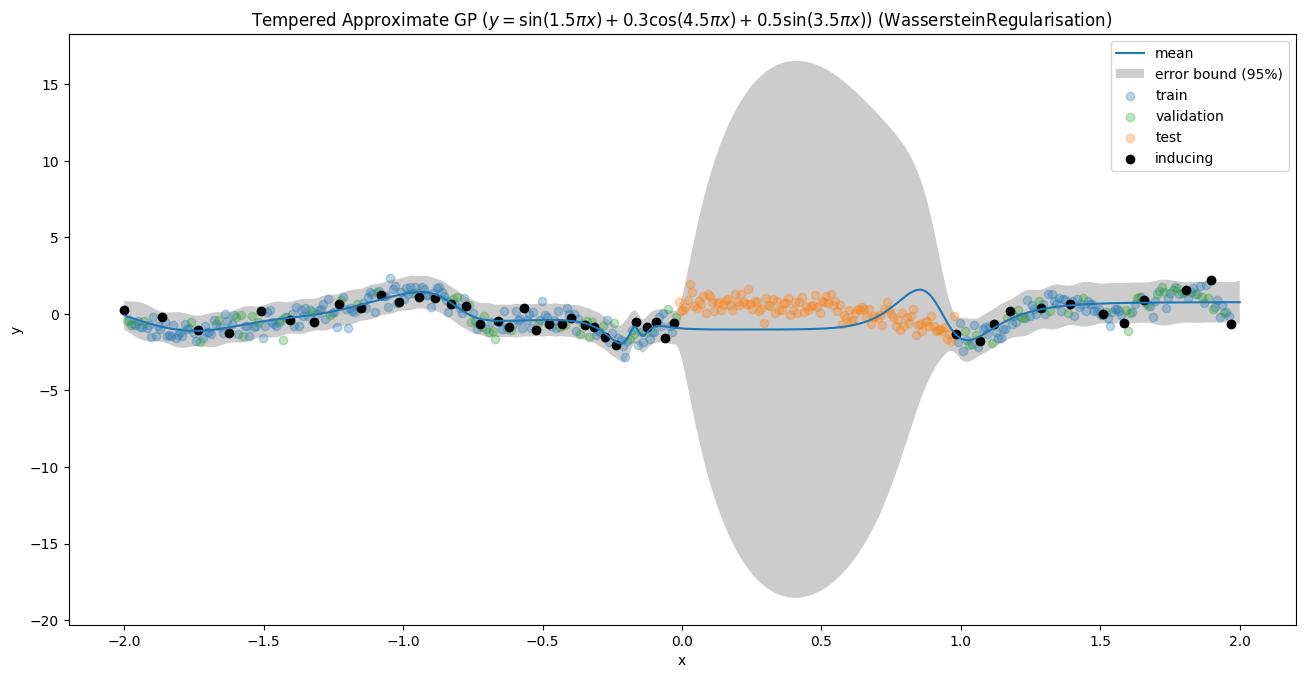
\includegraphics[width=0.9\linewidth]{experiments/regression/toy_curves/outputs/curve3/tempered-WassersteinRegularisation.png}
\end{minipage}%
\begin{minipage}{.5\textwidth}
  \centering
  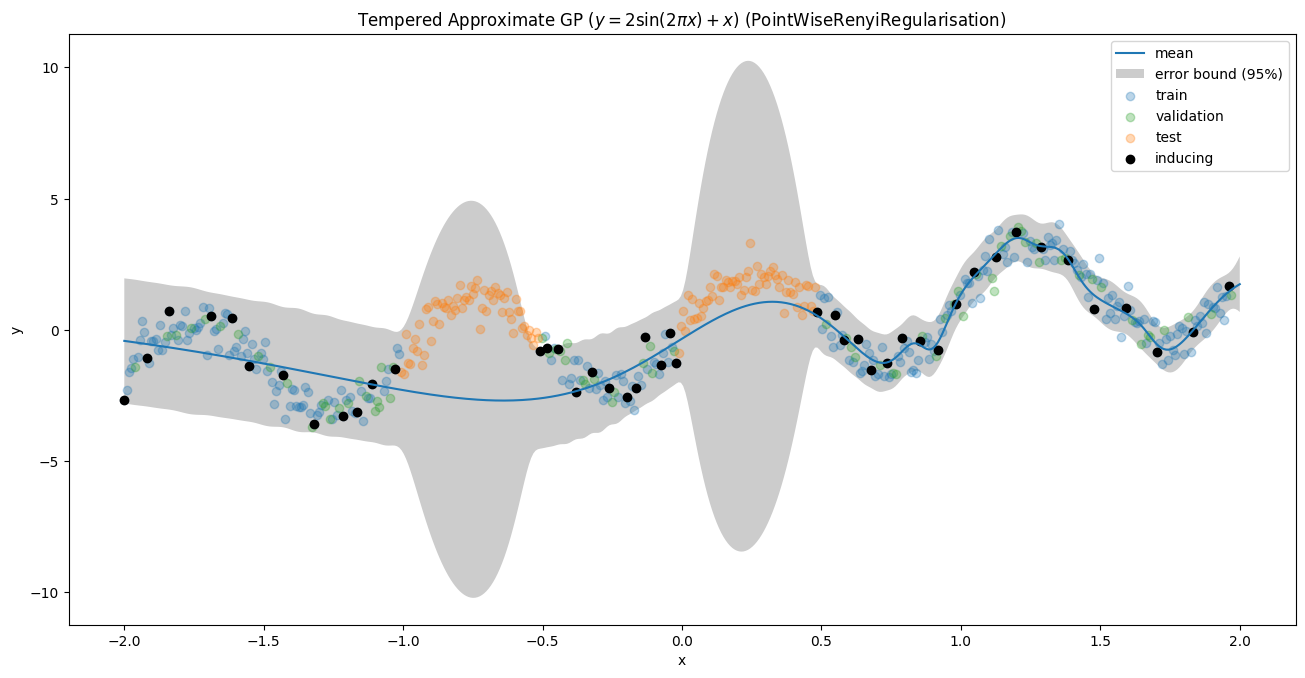
\includegraphics[width=0.9\linewidth]{experiments/regression/toy_curves/outputs/curve4/tempered-PointWiseRenyiRegularisation.png}
\end{minipage}
\caption{Example GVI-GPs for Regression}
\end{figure}
\subsection{Regression Results}

\subsection{Image Classification Results}

\newpage
\section{Future Work}
\subsection{NLP Named-Entity Recognition}
\jw{Putting pre-trained transformers in the mean and kernels.} 


\subsection{Inducing Points Selection}
\subsubsection{Not using actual data points}
\jw{Not selecting actual training points, but learning points that are most representative of the data? i.e. naively a convex combination of images, or weight params in a single layer NN.}
\subsubsection{Selecting in a Feature Space}
\jw{i.e. choosing inducing points from the feature representation of the data points from a NN feature extractor}


\newpage
\section{Conclusions}

\newpage
\bibliography{references}


\newpage
\appendix
\section{Appendix}

\end{document}